\documentclass[article]{jss}
%\usepackage{thumbpdf}

\author{Michael Lawrence\\
Iowa State University \And Duncan Temple Lang\\
University of California - Davis}

\title{\pkg{RGtk2}:\\A Graphical User Interface Toolkit for \proglang{R}}

\Plainauthor{Michael Lawrence, Duncan Temple Lang}
\Plaintitle{RGtk2: A Graphical User Interface Toolkit for R} 
\Shorttitle{RGtk2} 

\Abstract{
\pkg{RGtk2} is an \proglang{R} package for creating
a graphical user interface (GUI). It is a bridge between 
\proglang{R}  and \pkg{GTK+} 2.0, an open-source GUI toolkit written in \proglang{C}.
\pkg{RGtk2} supports the creation and manipulation of \pkg{GTK+} widgets and the
handling of user events. It also binds several libraries related to 
\pkg{GTK+}, including \pkg{Pango} (font rendering and text layout), \pkg{Cairo}
(2D vector graphics), and \pkg{Libglade} (\pkg{GTK+} GUI construction based on 
XML). The primary goal of \pkg{RGtk2} is complete control over \pkg{GTK+} and 
the other libraries via an interface that is consistent with \proglang{R} conventions.
From the technical perspective, this requires a complete and consistent
mapping of \proglang{C} functions and data structures of each API to \proglang{R}.
\pkg{RGtk2} allows the user to create and extend \pkg{GObject} classes. 
Basic and advanced examples of constructing 
GUI's with \pkg{RGtk2} are provided. The package is available from CRAN.
}

\Keywords{graphical user interface, GUI, R, GTK+}

\Address{Michael Lawrence\\
Department of Statistics\\
Iowa State University\\
Ames, IA, USA\\
E-mail: lawremi@iastate.edu\\
}

\begin{document}

\section{Introduction}

A graphical user interface (GUI) is a collection of objects called
widgets. A widget is a graphical element on a computer display that
communicates some information to the user. Examples of widgets include
labels, buttons, and scrollbars. Many widgets are also interactive
in that they accept input from the user, most often via a pointer
device or a keyboard. Pointing to a button and clicking with a mouse,
for example, performs the action associated with the button. Widgets
are often contained in other widgets, such as windows and tabbed notebooks.
Combining primitive widgets like labels and icons within containers
leads to more complex widgets, such as menus, toolbars, and combo
boxes. 

GUIs have been in common use since the 1970's and are the primary
means of interacting with modern operating systems like Microsoft
Windows, Mac OS, and Linux (in conjunction with the X Windows System).
Although a GUI is often more rigid than a text-based command line
interface (CLI) equivalent, novice users usually find a GUI to be
more intuitive and easier to learn.

When GUIs are constructed on top of the \proglang{R} platform \citep{R}, novice
users, such as biologists, are able to capitalize on the analytical functionality
of \proglang{R}, without the time expense of learning a programming language. 
For example, the \proglang{R} package \pkg{limmaGUI}
\citep{Limma} provides a GUI that guides a biologist through a microarray
data analysis task using \pkg{limma} and several other \proglang{R} packages from Bioconductor
\citep{bioconductor}, a collection of \proglang{R} packages for bioinformatics.
Even experienced \proglang{R} users might sometimes appreciate a GUI, such as when
manipulating and interacting with plots.

\pkg{RGtk2} provides \proglang{R} programmers with the ability to construct GUIs using
the \pkg{GTK+} cross-platform (Windows, Mac, and Linux) widget library \citep{GTK}.
The letters \emph{GTK} stand for the \emph{GIMP Tool Kit}, with the
word \emph{GIMP} recording the origin of the library as part of the
GNU Image Manipulation Program. \pkg{GTK+} 1.2 was bound to 
\proglang{R} by \pkg{RGtk} \citep{RGtk}, the predecessor
to \pkg{RGtk2}. \pkg{GTK+} was later largely refactored, bumping its version from 1.2 to 2.0.
The new 2.x series of \pkg{GTK+} is often referred to as \pkg{GTK2}, as
it is in this paper. Among other changes, \pkg{GTK2} brought many new widgets 
and integrated \pkg{GTK+} with several other libraries: \pkg{Pango} \citep{pango} 
for internationalized antialiased fonts and text layout, \pkg{Cairo} \citep{cairo}
for antialiased vector-based drawing, \pkg{ATK} \citep{atk} for accessibility
and \pkg{GdkPixbuf} \citep{gdkpixbuf} for images. \pkg{RGtk} was subsequently 
overhauled to become \pkg{RGtk2} to keep pace with \pkg{GTK+}. \pkg{RGtk2} adds 
bindings to the new features in \pkg{GTK2} and to the supporting libraries 
listed above. 

Several other GUI toolkits besides \pkg{GTK+} have been linked to \proglang{R}. The
most widely used is \pkg{tcl/tk} \citep{ousterhout,welch}, bound by the \pkg{tcltk} 
package \citep{Rnews:Dalgaard:2001a, Rnews:Dalgaard:2002}.
Bindings from \proglang{R} to \proglang{Java}, such as \pkg{rJava} \citep{rjava} 
and \pkg{SJava} \citep{sjava},
provide access to \proglang{Java} GUI toolkits, like \pkg{Swing} and \pkg{SWT}. The \pkg{wxWidgets}
library \citep{wxwidgets} has also been connected to \proglang{R}. The recently
created \pkg{Cocoa} package \citep{rcocoa} provides a binding to Cocoa,
the native widget toolkit for Mac OS X. A detailed comparison of these
solutions to \pkg{RGtk2} may be found in Section \ref{sec:comparison}.

We continue in the next section by outlining the basic features and 
concepts of \pkg{RGtk2}. This is followed by some examples of using 
\pkg{RGtk2} to construct simple GUIs.  The paper then moves into a more technical
domain, introducing the advanced features of the 
interface, including the creation of new types of widgets. Next, we compare 
\pkg{RGtk2} to existing \proglang{R} bindings to GUI toolkits. We then present
a highly technical description of the design and generation of
the interface, which is followed by a discussion of more general binding issues.
Finally, the conclusion mentions some real world applications of 
\pkg{RGtk2} and explores potential directions for future development.

\section{Basic Features and Concepts}\label{sec:basic-features}

The basic features of \pkg{RGtk2} are summarized below:

\begin{itemize}
\item Create and manipulate \pkg{GTK+} widgets by calling \proglang{R} functions.
\item Access properties of widgets with the \proglang{R} subset operators
('{\$}' and '{[}' and '{[}{[}')
\item Register \proglang{R} functions to be called in response to user 
interaction with a widget.
\item Introspect the widget class hierarchy and retrieve information on
the properties and signals for each type of widget.
\item Use additional libraries integrated with \pkg{GTK+} 2.0: \pkg{Cairo}, 
\pkg{Gdk}, \pkg{GdkPixbuf}, \pkg{Pango}, \pkg{ATK} and \pkg{Libglade}.
\item Embed \pkg{Cairo}-drawn (antialiased and alpha-blended) 
\proglang{R} graphics using the \pkg{cairoDevice} package.
\item Use \emph{RGtkDataFrame} to efficiently load and retrieve data.frames
to and from the \pkg{GTK+} table widget, \emph{GtkTreeView}. The complexity
of the data model is hidden behind the same syntax used for accessing data.frames.
\item Learn using the packaged demos and online R help that introduce the user to the
\pkg{RGtk} style.
\end{itemize}

The following paragraphs give further detail on these features.

\paragraph{Creating and Manipulating Widgets}

Creating an instance of a \pkg{GTK+} widget requires a single \proglang{R} 
function call. In \pkg{RGtk2}, the function names follow a ``camelBack'' 
capitalization scheme, so for example \emph{gtk\_window\_new}, as specified
by the \pkg{GTK+} \proglang{C} API, is collapsed to 
\emph{gtkWindowNew}, which is easier to type. Since \emph{gtkWindowNew} is a constructor,
\pkg{RGtk2} offers a wrapper function with a shorter name that matches the
class name with the first character in lower case, \emph{gtkWindow}. By default, 
\pkg{RGtk2} makes widgets visible upon construction.
The returned widget may be manipulated by passing it as the 
first argument to the appropriate \pkg{RGtk2} function. Below, we create an 
empty window and maximize it:

\begin{verbatim}
window <- gtkWindow("toplevel")
gtkWindowMaximize(window)
\end{verbatim}

In the above, the first parameter to the constructor of the window specifies
the type of the window. In this case, a top-level window is desired. The other
possible type is ``popup'', which is used, for example, for tooltips. The
set of possible window types is specified by what in \proglang{C} is known as
an \emph{enumeration}. Since enumerations are foreign to R, \pkg{RGtk2} accepts
string representations of enumeration values, like ``toplevel''. Every
enumeration has a corresponding \proglang{R} vector that maps the nicknames to 
the underlying numeric values. In the above case, the vector is named 
\emph{GtkWindowType}. It is rarely necessary to explicitly use the enumeration 
vectors; specifying the nickname will work in most cases.

For calling methods on widgets, \pkg{RGtk2} supports a syntax where the widget
variable is given first, followed by the \$ operator, then the method
name and its arguments. This is similar to the syntax used in \proglang{Java} and other 
object-oriented languages. For example, the \emph{gtkWindowMaximize(window)}
instruction from above may be shortened to \emph{window\$maximize()}. 
Although the two invocations do exactly the same thing, the second invocation is shorter.

Widgets that can contain other widgets are called \emph{containers}. There
are many different types of containers, but all of them support the addition
of child widgets using the \emph{gtkContainerAdd} function. We illustrate
this below by adding a button with the text ``Click Me!'' to the window.

\begin{verbatim}
button <- gtkButton("Click me!")
window$add(button) # or gtkContainerAdd(window, button)
\end{verbatim}

\paragraph{Accessing Widget Properties}

Each widget has a set of properties that partially describes its state. Examples
of properties include the title of a window, whether a checkbox is checked, and
the length in characters of a text entry box. The \proglang{R} subset functions, 
\emph{\$}, \emph{[}, and \emph{[[}, may be used to get the value 
of a widget property by name. Properties
may be set, given that they are writable, using the R assignment operator \emph{<-}.
The example below sets the title for the window created above, using this
familiar \proglang{R} syntax.

\begin{verbatim}
window$title <- "My First Window"
\end{verbatim}

\paragraph{Responding to User Interaction}

\pkg{GTK+} widgets report user interaction and other events by emitting 
\emph{signals}. In order to execute instructions in response to a signal, one
may connect an R function to a signal on a widget. The \emph{gSignalConnect}
function performs this connection. The following example will
cause ``Hello World!'' to be printed upon emission of the ``clicked'' signal
from the button in our window. The ``clicked'' signal is emitted when 
the user clicks the button with the mouse or other device.

\begin{verbatim}
gSignalConnect(button, "clicked", 
  function(widget) print("Hello world!"))
\end{verbatim}

\paragraph{The Widget Class Hierarchy}

\pkg{GTK+} 2.0 is based on an object-oriented framework known as \pkg{GObject},
which is class-based and uses single inheritance. A complete and quite technical
explanation of \pkg{GObject} is available in Section \ref{sec:primer}. 
A simpler explanation is given here. Each type of widget is a class that 
inherits from the base \emph{GtkWidget}
class. A widget class inherits every function, property and signal from each of
its parent classes. For example, the \emph{gtkContainerAdd} function used above
applies to the window, because \emph{GtkWindow}, like every type of container,
inherits from \emph{GtkContainer}.

\paragraph{Additional Library Support}

As mentioned above, \pkg{RGtk2} binds to several libraries in addition to 
\pkg{GTK+}. Although \pkg{GTK+} depends on all of these libraries, except \pkg{Libglade}, 
it is usually \emph{not} necessary to call them directly when constructing simple to 
intermediate GUIs. More detail on each library is presented below:

\begin{description}
\item [{\pkg{Cairo}:}] 2D vector graphics library with which \pkg{GTK+} widgets are
drawn. \pkg{Cairo} is likely useful outside of GUI construction, in that one
can draw vector graphics to off-screen surfaces like PNG, SVG, PS, and PDF files.
\item [{\pkg{GDK}:}] The low-level hardware access and drawing layer for \pkg{GTK+}.
It is most useful for raster-based drawing of graphical primitives like lines,
rectangles and circles and for handling raw mouse and keyboard events.
\item [{\pkg{GdkPixbuf}:}] Image manipulation library. Its features include 
rendering, scaling, and compositing. \pkg{GdkPixbuf} can read and write several image
formats, including JPEG, PNG, and GIF. Like \pkg{Cairo}, \pkg{GdkPixbuf} could
be used independently of a GUI for working with arbitrary graphics in \proglang{R}.
The \pkg{RGdkPixbuf} \citep{RGdkPixbuf} package bound the first generation of \pkg{GdkPixbuf}.
\item [{\pkg{Pango}:}] Renders and lays out antialiased, internationalized text.
It is most often used directly for embedding text in graphics.
\item [{\pkg{ATK}:}] Library for accessibility technologies. It allows \pkg{GTK+}
GUIs to be controlled by accessibility devices.
\item [{\pkg{Libglade}:}] Parses XML descriptions of \pkg{GTK+} user interfaces
and constructs the specified GUI. The XML descriptions are output from
\pkg{Glade}, which is a graphical tool for designing GUIs. The \pkg{RGtkGlade}
package \citep{RGtkGlade} bound the first generation of this library. As of 
\pkg{GTK+} 2.12.0, which includes native support for constructing widgets from 
XML descriptions, \pkg{Libglade} is essentially obsolete.
\end{description}

\paragraph{Embedding R Graphics}

It is possible, as one of the examples in the next section demonstrates,
to embed \proglang{R} graphics within an \pkg{RGtk2} GUI using the \pkg{cairoDevice}
package, which draws \proglang{R} graphics using \pkg{Cairo}. When \pkg{cairoDevice}
draws to the screen it is actually drawing to a type of \pkg{GTK+} widget called 
\emph{GtkDrawingArea}. Using the \emph{asCairoDevice} function, it is possible
to tell \pkg{cairoDevice} to draw to a \emph{GtkDrawingArea} widget created 
with \pkg{RGtk2}. The final step is to add the widget to an existing GUI, 
which will then contain \proglang{R} graphics. 
The code snippet below illustrates this process by adding a graphics device to a window:

\begin{verbatim}
library(cairoDevice)
window <- gtkWindow()
graphics <- gtkDrawingArea()
asCairoDevice(graphics)
gtkContainerAdd(window, graphics)
\end{verbatim}

\begin{figure}
\begin{center}
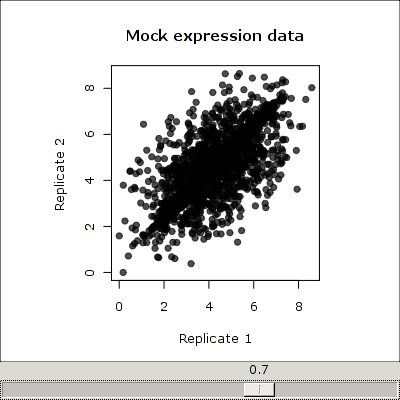
\includegraphics[scale=0.5]{demo-alpha-random-07-3}
\caption{\label{fig:rgtk2-demo-initial}Scatterplot of two microarray replicates,
with a slider widget underneath that controls the alpha level of the
points. This screenshot shows the initial alpha of $0.7$.}
\end{center}
\end{figure}

\begin{figure}
\begin{center}
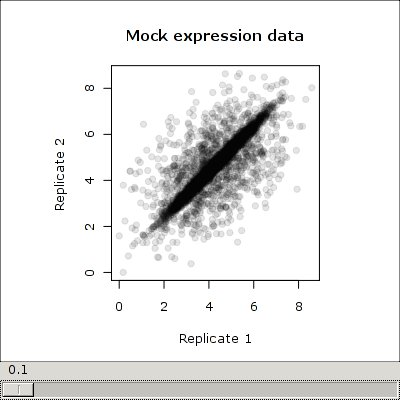
\includegraphics[scale=0.5]{demo-alpha-random-01-3}
\caption{\label{fig:rgtk2-demo-final}The same scatterplot from 
\ref{fig:rgtk2-demo-initial}, except the alpha has been set to to $0.1$.}
\end{center}
\end{figure}

\section{Examples}

Constructing a GUI may be conceptually divided into two basic steps.
First, one must create the individual widgets, specify their properties,
and organize them into containers. This defines the physical aspect
of the GUI: the appearance of the widgets and their spatial organization.
The second step defines the behavior or the logical aspect of the
interface. It involves registering handlers for signals that are emitted
by the widgets, for example in response to a user pressing a button.
The signal handlers encapsulate the logic beneath the interface. In
practice, these two steps are implemented simultaneously; their separation
is only conceptual, not physical, as we find in the following example.

\subsection{Embedded R Graphics}

In exploratory data analysis, it is often beneficial to integrate
a GUI with statistical graphics. As an example, we consider the contemporary
problem of visualizing micoarray data. The large number of genes leads
to a significant amount of overplotting when, for example, plotting
the expression levels from two chips in a scatterplot. One solution
to the problem of overplotting is alpha blending. However, choosing
the ideal alpha level may be time-consuming and tedious. Linking a
slider widget to the alpha level of an \proglang{R} scatterplot may accelerate
the search (See Figures \ref{fig:rgtk2-demo-initial} and \ref{fig:rgtk2-demo-final}). 

As a preliminary step, we use a 2D mixture distribution of correlated variables
to emulate expression values for two microarray chips. 
\begin{verbatim}
n <- 5000
backbone <- rnorm(n)
ma_data <- cbind(backbone+c(rnorm(3*(n/4),,0.1), rt(n/4, 80)), 
  backbone+c(rnorm(3*(n/4),,0.1), rt(n/4, 80)))
ma_data <- apply(ma_data, 2, function(col) col - min(col))
\end{verbatim}

\subsubsection{Creating the Widgets}

The first step towards making our GUI is to create the window that
will contain everything. 
\begin{verbatim}
win <- gtkWindow(show = F)
\end{verbatim}

Above, the first formal parameter to \emph{gtkWindow()}, which specifies the
type of the window, has been omitted, because the default (``toplevel'') is acceptable.  
In general, whenever a function parameter
has a reasonable default, \pkg{RGtk2} uses it as the default value in the
\proglang{R} wrapper. All widget constructors
in \pkg{RGtk2} accept a \emph{show} argument that if \emph{TRUE} (the default)
will make the widget visible immediately after construction.
In this case, we want to wait until the entire GUI is constructed. 

Next, we construct a drawing area in which the \proglang{R} graphics will be
drawn:
\begin{verbatim}
graphics <- gtkDrawingArea()
\end{verbatim}

Now that we have a widget for displaying \proglang{R} graphics, we need the slider
that controls the alpha level. The slider, a \emph{GtkHScale}, is created
with to range from 0.1 to 1.0, with a step size of 0.1. The \emph{GtkHScale}
class has two constructors, \emph{gtkHScaleNew} and \emph{gtkHScaleNewWithRange}.
The convenience constructor \emph{gtkHScale} wraps both of them by
merging the two parameter lists into its own.
\begin{verbatim}
slider <- gtkHScale(min=0.1, max=1.00, step=0.1)
\end{verbatim}

\subsubsection{Connecting a Callback}

The slider needs to be linked to the plot. This is achieved by connecting
an \proglang{R} callback to the ``value-changed'' signal of the slider. The callback,
\emph{scale\_cb}, replots the microarray data, \emph{ma\_data}, using
an alpha level equal to the current value of the slider. 
\begin{verbatim}
scale_cb <- function(range) 
  plot(ma_data[,1], ma_data[,2], col = rgb(0, 0, 0, range$getValue()),
    xlab = "Replicate 1", ylab = "Replicate 2", 
    main = "Mock expression data", pch = 19)
gSignalConnect(slider, "value-changed", scale_cb)
\end{verbatim}

\subsubsection{Packing the Widgets}

The next steps are to add the drawing area and the slider to the
window and then to show the window on the screen. Although the window is a
container, it inherits from \emph{GtkBin}, meaning that it can hold only
a single child widget. The most common containers for packing multiple widgets
are the subclasses of \emph{GtkBox}: \emph{GtkVBox} for vertical stacking and
\emph{GtkHBox} for horizontal stacking. Both the drawing
area and slider are packed into the vertical stacking box,
\emph{GtkVBox}, so that the drawing area is on top of the slider. The third and 
fourth arguments to the \emph{gtkBoxPackStart} function govern how the
space of the container is allocated to the packed child. The first of the two
is the \emph{expand} parameter, which if \emph{TRUE} causes the space allocated
for the child to expand against the spaces for the other children. Any child
that is packed with \emph{expand} as \emph{FALSE} will give up its available
space until its minimum size request is reached. All children packed with
\emph{expand} as \emph{TRUE} will have equal available space. The second is
the \emph{fill} parameter, which indicates whether the child widget should try to
fill all of its available space. The final parameter is the minimum amount of 
spacing, in pixels, that should be placed between the child and its adjacent siblings.
Here, we would like the graphics to take up all space not consumed by the slider,
so the graphics device is packed to \emph{expand} and \emph{fill}, while the
slider is not.
\begin{verbatim}
vbox <- gtkVBox()
vbox$packStart(graphics, TRUE, TRUE, 0)
vbox$packStart(slider, FALSE, FALSE, 0)
win$add(vbox)
win$setDefaultSize(400,400)
win$showAll() 
\end{verbatim}

Now that the window is visible on screen, we can instruct \proglang{R} to draw
its graphics to the drawing area. The Cairo graphics device, provided by the
\pkg{cairoDevice} package, is embeddable
into \pkg{RGtk2} interfaces and also satisfies our requirement for alpha
blending. The \emph{asCairoDevice} function
converts the drawing area created above to an \proglang{R} graphics device. 
\begin{verbatim}
require(cairoDevice)
asCairoDevice(graphics)
par(pty = "s")
\end{verbatim}

Finally, the value of the slider is initialized to 0.7, which in turn
activates the callback, generating the initial plot. The initial state
of the interface is shown in Figure \ref{fig:rgtk2-demo-initial}.
Figure \ref{fig:rgtk2-demo-final} shows the plot after the slider has been
moved to set the alpha at 0.1.
\begin{verbatim}
slider$setValue(0.7)
\end{verbatim}

\subsection{Requesting Input from the User}\label{sec:dialog-example}

Applications frequently need to request immediate input from the user. This is
usually done with a special type of window called a \emph{dialog}. All dialogs
in \pkg{GTK+} are based on the \emph{GtkDialog} widget. In this example,
we will create a dialog that asks whether the user really intends
to quit an application. Although we could build such a dialog using \emph{GtkDialog}
directly, \emph{GtkMessageDialog}, an extension of \emph{GtkDialog}, saves 
typing for simple queries. The dialog is constructed with a single function call:
\begin{verbatim}
dialog <- gtkMessageDialog(main_application_window, "destroy-with-parent", 
  "question", "yes-no", "Do you really want to quit?")
\end{verbatim}
In the above invocation, the first parameter indicates the parent window for
the dialog. It is assumed that the main window of the application is stored 
as \emph{main\_application\_window}. The second parameter indicates that
the dialog should be destroyed if its parent, the main window, is destroyed.
The next parameter indicates that this is a ``question'' dialog, which causes
the dialog to display a question mark icon to the left of the text. The 
predefined set of buttons, in this case consisting of ``Yes'' and ``No'', 
is specified by the next parameter. The final parameter specifies the message text.

It is desirable for this dialog to be \emph{modal}, meaning that the focus
is restricted to the dialog window until the user responds to the question. By
invoking the \emph{gtkDialogRun} function, the dialog becomes modal and execution
is blocked until the user gives a response, which may be retrieved from the 
dialog with \emph{gtkDialogGetResponse}. The call to \emph{gtkWidgetDestroy}
closes the dialog window and renders it unusable.
\begin{verbatim}
dialog$run()
if (dialog$getResponse() == GtkResponseType["yes"])
 quit_application()
dialog$destroy()
\end{verbatim}
The reference to \emph{GtkResponseType} above is one of the rare cases in which
it is necessary to access an enumeration vector to retrieve the numeric value
for a nickname. The reason for this is that \emph{gtkDialogGetResponse} returns
a plain numeric value, which makes sense if one considers the infinite number
of possible responses from a generic dialog. In this case, it is known from
the documentation of \emph{GtkMessageDialog} that the value corresponding to
the user clicking the ``Yes'' button will equal the ``yes'' value in \emph{GtkResponseType}.

\subsection{Presenting Options to the User}
% toggle button, radio buttons, combo box
It is often necessary to present the user with a set of options that help
define the behavior of an application. The simplest option is binary and is
usually represented by a checkbox. In \pkg{GTK+}, the checkbox is known as
the \emph{GtkCheckButton}. In the snippet below, we add a check button
to the quit confirmation dialog created above. The area above the buttons in the 
\emph{GtkDialog} is contained within a \emph{GtkVBox} that may be accessed
as if it were a property named \emph{vbox}.
\begin{verbatim}
check <- gtkToggleButton("Quit R, as well")
dialog$vbox$add(check)
\end{verbatim}

When an option has multiple choices, a check button is no longer adequate. A
simple extension is to create a set of toggle buttons where only one button
may be active at once. The buttons in this set are known as \emph{radio buttons}.
Below, we create a new dialog that asks the user to pick from three shapes.
When each radio button is created, it needs to be given the existing buttons
in the group. For creating the first button, \emph{NULL} should be passed as the group.
\begin{verbatim}
dialog <- gtkMessageDialog(NULL, "destroy-with-parent", 
  "question", "ok-cancel", "Which shape would you like?")
shapes <- c("Square", "Circle", "Hexagon")
radio_buttons <- NULL
for (shape in shapes)
  radio_buttons <- c(radio_buttons, gtkRadioButton(radio_buttons, shape))
sapply(radio_buttons, dialog$vbox$add)
\end{verbatim}

As the number of options increase, however, radio buttons tend to consume too 
much space. In this case, a drop down menu, known as \emph{GtkComboBox} in
\pkg{GTK+}, may be appropriate. The following snippet illustrates its use:
\begin{verbatim}
dialog <- gtkMessageDialog(NULL, "destroy-with-parent", 
  "question", "ok-cancel", "Which shape would you like?")
shapes <- c("Square", "Circle", "Hexagon", "Octagon", "Dodecagon")
combo <- gtkComboBoxNewText()
combo$show()
sapply(shapes, combo$appendText)
dialog$vbox$add(combo)
\end{verbatim}

These are just a few of the simpler ways of presenting choices to the user. 
A more complex application may employ, for example, a menubar
and a toolbar, as demonstrated in the next example.

\subsection{A Simple Spreadsheet Application}\label{sec:spreadsheet-example}

This example demonstrates how one might construct a reasonably complex
application using \pkg{RGtk2}. We aim to build a viewer of R \emph{data.frame}s that
is capable of sorting and filtering. It should also be able to load and save
a \emph{data.frame} to and from a CSV file. The actions for loading, saving, and quitting
should be available in the menubar and toolbar. We begin by creating the
main window, defining the actions and bundling them into a \emph{GtkActionGroup}.
\begin{verbatim}
main_window <- gtkWindow(show = FALSE)
main_window$setDefaultSize(600,600)
open_cb <- save_cb <- quit_cb <- function(widget, window) 
{
  # these callbacks are left as a challenge to the reader
  # see help(GtkFileChooserDialog) for file selection
}
actions <- list(
  list("FileMenu", NULL, "_File"), 
  list("Open", "gtk-open", "_Open File", "<control>O", 
    "Select a CSV file to load as a spreadsheet", open_cb),
  list("Save", "gtk-save", "_Save", "<control>S", 
    "Save the current spreadsheet to a CSV file", save_cb),
  list("Quit", "gtk-quit", "_Quit", "<control>Q", "Quit the application", quit_cb)
)
action_group <- gtkActionGroup("spreadsheetActions")
action_group$addActions(actions, main_window)
\end{verbatim}
Each action is defined with a list, containing the action name, stock ID,
label, keyboard shortcut, tooltip, and callback. This is an example of 
high-level type conversion, see Section \ref{sec:high-level-conversion} for
a technical explanation. The first action will serve as 
the menu shell for the rest of the actions. Since it performs no
function, it is not necessary to specify all of the fields. Next, we specify
the layout of the menubar and toolbar using the actions defined above, using
an XML description.
\begin{verbatim}
layout <- paste(
"<ui>",
"  <menubar name='Menubar'>",
"    <menu action='FileMenu'>",
"      <menuitem action='Open'/>",
"      <menuitem action='Save'/>",
"      <separator/>",
"      <menuitem action='Quit'/>",
"    </menu>",
"  </menubar>",
"  <toolbar name='Toolbar'>",
"    <toolitem action='Open'/>",
"    <toolitem action='Save'/>",
"    <toolitem action='Quit'/>",
"  </toolbar>",
"</ui>", sep="\n")
\end{verbatim}
Next, we create a \emph{GtkUIManager} and use it to create the menubar and
toolbar widgets given the action group and layout.
\begin{verbatim}
ui_manager <- gtkUIManager()
ui_manager$insertActionGroup(action_group, 0)
main_window$addAccelGroup(ui_manager$getAccelGroup()) # so shortcuts work
ui_manager$addUiFromString(layout)
menubar <- ui_manager$getWidget("/Menubar")
toolbar <- ui_manager$getWidget("/Toolbar")
\end{verbatim}
In order to handle multiple spreadsheets at once, we will use a special type
of container called the \emph{notebook}. A notebook only shows a single widget
(and its children) at once. The user may choose the visible widget by 
clicking on the corresponding tab on the border of the notebook. Below,
we create the notebook and add it, along with the menubar and toolbar, to the
window, through a \emph{GtkVBox}.
\begin{verbatim}
notebook <- gtkNotebook()
notebook$setTabPos("bottom") # like Excel
vbox <- gtkVBox(FALSE, 0)
vbox$packStart(menubar, FALSE, FALSE, 0)
vbox$packStart(toolbar, FALSE, FALSE, 0)
vbox$packStart(notebook, TRUE, TRUE, 0)
main_window$add(vbox)
main_window$show()
\end{verbatim}
Next, we define a function that will add a spreadsheet page to the notebook.
This will use the \emph{RGtkDataFrame} utility that allows
the \emph{GtkTreeView} (a combined tree and table widget) to use an \proglang{R}
\emph{data.frame} as its data model. This model is proxied by a \emph{GtkTreeModelFilter}
and \emph{GtkTreeModelSort} so that the table is filterable, according to
a specified logical (boolean) column in the model, and sortable. 
The table is added to a \emph{GtkScrolledWindow},
a container widget that provides a scrolled view of its child when the child
requests too much space.
At the bottom of the table will be a text entry
box for the user to enter an \proglang{R} subset expression that will filter the table.
\begin{verbatim}
load_spreadsheet <- function(df, name = deparse(substitute(df)))
{
  df <- cbind(rownames = rownames(df), df)
  filter_df <- cbind(filter = TRUE, df)
  model <- rGtkDataFrame(filter_df)
  filter_model <- gtkTreeModelFilterNew(model)
  filter_model$setVisibleColumn(0)
  tree_view <- gtkTreeView(gtkTreeModelSort(filter_model))
  tree_view$setHeadersClickable(TRUE) # sort by clicking on column header
  if (is.null(gtkCheckVersion(2,10,0))) # check for API after version 2.8.x
    tree_view$setGridLines("both")
  append_tree_view_column <- function(j)
  {
    column <- gtkTreeViewColumn(colnames(df)[j], gtkCellRendererText(), text = j)
    column$setSortColumnId(j)
    tree_view$appendColumn(column)
  } # add view columns for each data column
  sapply(seq_len(ncol(df)), append_tree_view_column)
  
  entry <- gtkEntry() # for filter expression
  subset_table <- function(entry)
  { # update column used by filter according to logical expression
    model[,"filter"] <- eval(parse(text=entry$text), df)
  }
  gSignalConnect(entry, "activate", subset_table)
  hbox <- gtkHBox(FALSE, 5)
  hbox$packStart(gtkLabel("Filter expression:"), FALSE, FALSE, 0)
  hbox$packStart(entry, TRUE, TRUE, 0)
  
  vbox <- gtkVBox(FALSE, 5)
  scrolled_window <- gtkScrolledWindow()
  scrolled_window$add(tree_view) # support scrolling for the table
  vbox$packStart(scrolled_window, TRUE, TRUE, 0)
  vbox$packStart(hbox, FALSE, FALSE, 0)
  
  notebook$appendPage(vbox, gtkLabel(name))
}
\end{verbatim}
An example of using the above function to add a spreadsheet is given below:
\begin{verbatim}
data(mtcars)
load_spreadsheet(mtcars)
\end{verbatim}
This application is obviously missing many important features. For example, 
there is no easy way to return to the complete \emph{data.frame} after subsetting, and
it is not possible to edit the cells. The reader could try to add such features
as an exercise.

\section{Advanced Features}

\subsection[A GObject Primer]{A \pkg{GObject} Primer}\label{sec:primer}

The advanced features of \pkg{RGtk2} involve working directly with
\pkg{GObject}, a \proglang{C} library for object-oriented programming. 
\pkg{GObject} sits at the core of \pkg{GTK+} and other 
open-source projects, including the \pkg{GNOME} \citep{GTK} and \pkg{XFCE} 
\citep{xfce} desktops and the \pkg{GStreamer} multimedia framework \citep{gstreamer}.
it is based on \pkg{GLib}, a library of generic utilities for
writing applications in \proglang{C}.
\pkg{GObject} is composed of several modules: \emph{GType},
\emph{GSignal}, \emph{GParamSpec}, and the base \emph{GObject} 
class, among others. Each of mentioned modules is described in further detail 
below. For reference, please see \citep{gobject}.

\subsubsection{GType}

\emph{GType} is the most fundamental module of \pkg{GObject}. It supports runtime 
registration and introspection of types. The
main commonality between all GTypes, as they are called, is that they define
a method for copying their values. This allows generic memory management for
every value with a GType. Those GTypes that directly define a copy mechanism,
instead of inheriting one, are known as \emph{fundamental} types.
GTypes are further classified by whether they are classed and whether they are
instanciable. 

Fundamental types that are non-classed and non-instanciable 
include ``primitive'' types like integers and strings, as well as \emph{GBoxed}.
Types that extend \emph{GBoxed} are able to register functions for their
copying and freeing. This facilitates creating a GType for an ordinary 
\proglang{C} structure. For example, \pkg{RGtk2} registers a boxed type for 
the \emph{SEXP} structure of \proglang{R}. 

The fundamental \emph{GObject} type is both classed and instanciable. Classed 
types are associated with a class structure, which is prefixed by the class structure 
of its parent class, with \emph{GTypeClass} at the beginning. Thus, only single
inheritance is allowed in \pkg{GObject}.
The class structure contains class-wide fields, including function pointers
called \emph{virtual functions} that may be overriden by changing
the value of the corresponding field in the class structure during intialization.
This is the primary mechanism in \pkg{GObject} for changing object behavior through
inheritance. For convenience, wrappers are normally implemented for virtual
functions that are meant to be public. The values of instanciable types are 
structures that, like class structures, are prefixed by the instance structure
of the parent type, with \emph{GTypeInstance} at the top. 
This allows inheritance of instance fields. 

\emph{GTypeInterface} is an example of a classed but non-instanciable GType.
An interface in \pkg{GObject} is specified through the
virtual functions declared in its class structure. It is possible to register 
an interface against a classed and instanciable type, like \emph{GObject}. As
a result, the type is required to provide values (implementations) for the 
virtual methods declared by the interface.
Every derivative of \emph{GTypeInterface} must extend \emph{GTypeInterface} directly, 
so there is no inheritance between interfaces in \pkg{GObject}. However, an 
interface can be made to \emph{require} the implementation of one or more other 
interfaces by any type that implements it.

Two other fundamental, classed, non-instanciable types are \emph{GEnum} and 
\emph{GFlags}. The \emph{GEnumClass} stores metadata about a particular
enumeration, such as the names and nicknames of its values. \emph{GFlags} is
similar as it represents an enumeration with values that are powers of two, 
so that they may be combined with a bitwise \emph{or} operation.

\subsubsection{GSignal}

One of the defining characteristics of \pkg{GObject} is its emphasis on
\emph{signals}, which were introduced earlier in this paper in the context of
notification of user events in a \pkg{GTK+} GUI. Technically,
any instance of a GType can have registered signals, but they are usually 
discussed only in the context of objects. Each \emph{signal} is defined
by its name and the types of its arguments and return value. A class inherits
signals from its parents.

\subsubsection{The GObject Base Class}

\emph{GObject} is the classed and instanciable type provided by the \pkg{GObject}
library. Although it is possible to create a new base object class on top of
\emph{GType}, virtually all libraries based on \pkg{GObject} use the 
\emph{GObject} class as the base for their class hierarchies. 

The key feature of the \emph{GObject} class, from the perspective of the 
\pkg{RGtk2} user, are \emph{properties}. Properties may be described as 
introspectable and encapsulated public fields. Like fields, properties are 
inherited. They support automated validation 
of their values at runtime, and a change in a property value emits the 
\emph{notify} signal from its instance, allowing objects to respond
to changes in the state of other objects. It is possible to control whether a 
property is readable, writeable, and more. Depending on its options,
one may be able to or even restricted to set a property at construction time, 
using the generic \emph{GObject} constructor, \emph{gObject()}. Properties are 
inherited.

A property is defined by a \emph{GParamSpec} structure that specifies a name, 
nickname, description, value GType, and other options. There are subclasses of 
\emph{GParamSpec} for particular GTypes that permit specification of further 
constraints. For example, \emph{GParamSpecInt} is specific to integers and can be
configured to restrict its valid range of integer values between a minimum and maximum.
Many \emph{GParamSpec} subclasses also permit default values.

\subsection[Interfacing With External GObject-based Applications]{Interfacing With External \pkg{GObject}-based Applications}

Much of the \pkg{RGtk2} functions that were developed to support the
creation of GUIs using \pkg{GTK+} are also applicable to other libraries
and applications based on \pkg{GObject}. There are several such packages of
interest to staticians, including \pkg{Gnumeric}, a spreadsheet application, and
\pkg{GGobi}, software for multivariate interactive graphics. The \pkg{rggobi}
package \citep{rggobi} provides a high-level interface to \pkg{GGobi} from 
\proglang{R}. Although it is somewhat hidden, \pkg{rggobi} objects are 
\emph{externalptr}s that reference the underlying \pkg{GGobi} objects, which
extend \emph{GObject}. \pkg{RGtk2} uses the same \proglang{R} representation, so
many \pkg{RGtk2} functions can operate on \pkg{rggobi} objects.

As an example, we consider the problem of displaying an \proglang{R} plot in
response to a user ``identifying'' a point in a \pkg{GGobi} plot with the mouse.
When a \pkg{GGobi} point is identified, the main \pkg{GGobi} context emits
the ``identify-point'' signal. If we connect an \proglang{R} function to
``identify-point'' signal, using \emph{gSignalConnect}, the function will be
executed whenever a point is identified. The code below illustrates this process:
\begin{verbatim}
# still need to add this example
\end{verbatim}
Since the \pkg{GGobi} GUI is based on \pkg{GTK+}, it is possible to embed 
\pkg{GGobi} displays into \pkg{RGtk2} GUIs, but that interface is still in flux
and will not be detailed here.

\subsection[Defining GObject Classes]{Defining \pkg{GObject} Classes}

All of the above examples utilize objects that are implemented in \proglang{C}.
\pkg{RGtk2} also supports the creation of \emph{GObject}-derived classes from within
\proglang{R}. The programmer may define methods, fields, virtual function
overrides, signals, properties and an initialization function. 
Methods and fields may be encapsulated at the public, protected or private level.
Public members may be accessed by any code given an instance of the class, 
while protected members are restricted to methods belonging to the same class or
a subclass. Access to private members is the most restricted as they are only 
available to methods in the same class. Any 
virtual function defined by an inherited class or registered interface may be 
overriden, and it is possible to chain up to parent handlers. Any public or 
protected method may be overridden (within \proglang{R}) as if it were a virtual
function. The definitions of signals and properties may refer to any GType by name. 
The names of primitive \proglang{R} types, like \emph{integer} and \emph{character} 
are mapped to the corresponding GType if available. It is also possible to specify the 
\emph{RGtkSexp} type; its values are left as native \proglang{R} objects instead
of being converted to a \proglang{C} type, allowing the storage of complex 
\proglang{R} values like S4 objects. The initialization function is executed 
whenever the class is instanciated. The \emph{gClass} function registers the 
class, given the class name, the name of the parent class, and the class 
definition. After registration, instances may be
created using the \emph{gObject} function.

The class definition is an \proglang{R} \emph{list} that specifies the
methods, fields, virtual function overrides, signals, properties, and
initialization function for the class. The name of a list element specifies
its role in the definition. For methods and fields, there is a 
list for each level of encapsulation. The lists are named
according to their level: \emph{.public}, \emph{.protected} or \emph{.private}. 
The functions for the methods and the initial assignments for the fields should
be placed inside the appropriate list. The name of a member in the list 
serves as its identifier. A virtual function override is a function that is 
placed in a list with the same name as the class that defines the virtual 
function. The name of override in that list should match the name of the virtual 
function. The list named \emph{.signals} contains lists that each define
a signal for the class. The properties are defined by \emph{GParamSpec}
structures that may be created using the \emph{gParamSpec} function. These
are stored in a list named \emph{.props}. Finally, the initialization function
is stored in the class definition list as \emph{.init}. Further details
are available in the \proglang{R} help for the \emph{gClass} function.

The example below illustrates the definition of a new \emph{GObject}-derived
class by revisiting the first example, involving the embedded plotting of 
microarray data. The slider in that example controls the alpha level of the
points in the scatterplot in a linear fashion. Given the large amount of
overplotting, the alpha level does not have a strong visual effect until it
approaches its lower limit. One may desire greater control in this region,
without limiting the range of the slider. 

A possible solution would be to map the slider value to an alpha value using a 
non-linear function. All that is
really required is to change the slider callback so that it computes the
alpha value as a non-linear function of the slider value. However, the 
label on the slider would be inaccurate; it would still report the original value.
Overriding this is possible by connecting to the ``format-value'' signal on
the \emph{GtkScale} class. Let us assume, however, that we would like to create
a reusable type of slider that mapped its value using a specified \proglang{R} expression.
Below is our invocation of \emph{gClass}, including the class definition list.
\begin{verbatim}
tform_scale_type <- gClass("RTransformedHScale", "GtkHScale", list(
  .props = list(
    gParamSpec("R", "expr", "e", "Transformation of scale value",
      default.value = expression(x))
  ),
  .public = list(
    getExpr = function(self) self["expr"],
    getTransformedValue = function(self) self$transformValue(self$value)
  ),
  .private = list(
    transformValue = function(self, x) eval(self$expr, list(x = x))
  ),
  GtkScale = list(
    format_value = function(self, x)
      as.character(self$transformValue(x))
  )
))
\end{verbatim}
The \emph{RTransformedHScale} extends \emph{GtkHScale}, the horizontal slider.
It defines a single property of type \emph{RGtkSexp}, or ``R'' for short, named
``expr'', with a default value of ``expression(x)''. For \emph{RGtkSexp}
properties, it is possible to specify the underlying \proglang{R} type for
validation purposes. In this case, that type is inferred from the default
value, which is of mode \emph{expression}. The ``any'' type allows a property
to hold any \proglang{R} type. The next step is to create an instance
of the type and to register a handler on the ``value-changed'' signal that
will draw the plot using the transformed value as the alpha setting.
\begin{verbatim}
adj <- gtkAdjustment(0.5, 0.15, 1.00, 0.05, 0.5, 0)
s <- gObject(tform_scale_type, adjustment = adj, expr = expression(x^3))
gSignalConnect(s, "value-changed", function(scale) {
  plot(ma_data, col = rgb(0,0,0,scale$getTransformedValue()),
    xlab = "Replicate 1", ylab = "Replicate 2", 
    main = "Expression levels of WT at time 0",  pch = 19)
})
\end{verbatim}
The expression $x^3$ is set on the ``expr'' property at construction. The
signal handler now calls the new \emph{getTransformedValue} method, instead
of \emph{getValue} as in the original version. This final block of code
completes the example:
\begin{verbatim}
win <- gtkWindow(show = F)
da <- gtkDrawingArea()
vbox <- gtkVBox()
vbox$packStart(da)
vbox$packStart(s, FALSE)
win$add(vbox)
win$setDefaultSize(400,400)

require(cairoDevice)
asCairoDevice(da)

win$showAll()
par(pty = "s")
s$setValue(0.7)
\end{verbatim}

\section[Comparison of RGtk2 to other R GUI toolkit bindings]{Comparison of \pkg{RGtk2} to other \proglang{R} GUI toolkit bindings}\label{sec:comparison}

There are many different ways to construct a GUI from \proglang{R}. The great
majority of \proglang{R} GUIs rely on the \pkg{tcltk} package that binds 
\proglang{R} to \pkg{tcl/tk} \citep{ousterhout,welch}, a mature light-weight cross-platform
widget library. The \pkg{tcltk} package \citep{Rnews:Dalgaard:2001a, Rnews:Dalgaard:2002} 
is bundled with the core distribution of 
\proglang{R}. This means that developers can usually count on its availability, which
is more convenient than depending on \pkg{RGtk2}, which requires the user
to install \pkg{RGtk2}, \pkg{GTK+}, and all of the libraries on which \pkg{GTK+}
depends. The small footprint of \pkg{tcl/tk} likely delivers better performance in
terms of speed and memory than \pkg{GTK+} in many circumstances. \pkg{tcl/tk}
also offers some features that currently \pkg{GTK+} lacks, the canvas widget
being one example.

Unfortunately, \pkg{tcl/tk} development is slow and the library is beginning
to show its age. It lacks many of the widgets present in \pkg{GTK+} and
other modern toolkits, such as tree tables, progress bars, and autocompleting
text fields. \pkg{tcl/tk} widgets are often less sophisticated than their
\pkg{GTK+} counterparts. For example, a \pkg{GTK+} menu is able to be torn off
as an independent window and the \pkg{GTK+} file chooser supports the storage
of shortcuts. \pkg{tcl/tk} also lacks theme support, so it is not able to
emulate native look and feels. There is no existing means
for constructing \pkg{tcl/tk} GUIs from XML descriptions, like \pkg{Libglade}
\citep{libglade} for \pkg{GTK+}. Also, \pkg{tcl/tk} is not object-oriented,
and it is not possible to override the fundamental behavior of widgets.
While it is possible to build so-called ``megawidgets'' on top of existing
\pkg{Tk} widgets, this is not the same as creating new \emph{GtkWidget}-derived
classes with \pkg{RGtk2}. Moreover, the design goals of the \pkg{tcltk} package
differ from those of \pkg{RGtk2}, in that \pkg{tcltk} aims to expose much of the 
functionality of the \proglang{Tcl} language to the \proglang{R} programmer, while 
\pkg{RGtk2} is a binding to a collection of \proglang{C} libraries that attempts 
to hide \proglang{C}-specific details.

The \pkg{tcltk2} package \citep{tcltk2} is an attempt to overcome some
of the limitations of the \pkg{tcltk} package by binding the \pkg{Tile} extension
\citep{tcltk-tile} of \pkg{tcl/tk}. Tile adds support for themes, allowing
emulation of native widgets and prettier GUIs, as well as new widgets
like a tree table and progress bar. However, Tile still lags behind
\pkg{GTK+}. For example, the \pkg{GTK+} tree table allows the embedding of images,
check boxes, and combo boxes, while the \pkg{Tile} one does not.

There are several bindings from \proglang{R} to \proglang{Java}, including \pkg{SJava} \citep{sjava}
and \pkg{rJava} \citep{rjava}. \pkg{SJava} supports creating
new \proglang{Java} widget classes from \proglang{R}, like \pkg{RGtk2} does for 
\pkg{GTK+} and its \pkg{GObject} classes. There are two major GUI libraries for 
\proglang{Java}: \pkg{Swing} and \pkg{SWT}. The features
of \pkg{Swing} and \pkg{SWT} are comparable to those of \pkg{GTK+}. \pkg{Swing} is included
in the \proglang{Java} platform and is far more popular than \pkg{SWT}. Both \pkg{Swing}
and \pkg{SWT} differ from \pkg{GTK+} in terms of API design, due in part
to the differences between \proglang{C} and \proglang{Java}. \pkg{SWT} differs 
from \pkg{Swing} and \pkg{GTK+} in that it provides a common API with 
platform-specific implementations based on native widgets, which perfectly 
preserves the look and feel of each platform, without resorting to emulation. 
This differs from the \pkg{GTK+} and \pkg{Swing} approach of providing exactly 
the same widgets on all platforms, leaving the look and feel to theme engines.

Another library that takes the \pkg{SWT} approach is \pkg{wxWidgets} \citep{wxwidgets},
written in \proglang{C++}. \pkg{GTK+} serves as its {}``native'' implementation on
Linux. The first binding from \proglang{R} to \pkg{wxWidgets} was the now defunct \pkg{wxPython}
package that leveraged \pkg{RSPython} to access the \proglang{Python} binding to \pkg{wxWidgets}.
Fortunately there is a new binding to \pkg{wxWidgets}, known as \pkg{RwxWidgets}
\citep{RwxWidgets}. \pkg{wxWidgets} is somewhat restricted by the combined
limitations of its underlying native libraries, so it is not able
to offer the fine-grained control of \pkg{GTK+}. \pkg{wxWidgets} also lacks integrated
2D vector graphics. Furthermore, the \pkg{RwxWidgets} package does not yet
bind to an XML GUI builder like \pkg{Libglade}, nor does it support
extending wxWidgets from \proglang{R}. However, \pkg{wxWidgets} does provide some
features that do not exist yet in base \pkg{GTK+}, such as HTML display
and a dockable window framework. 

The \proglang{R} package \pkg{gWidgets} \citep{gwidgets} is an abstraction library similar to
\pkg{wxWidgets} and \pkg{SWT} in that it supports multiple toolkit backends.
Since \pkg{gWidgets} is written in \proglang{R}, these backends rely on 
bindings to the external toolkits. So far, there are two backends for 
\pkg{gWidgets}, \pkg{gWidgetsRGtk2}, based on \pkg{RGtk2}, and \pkg{gWidgetsJava},
based on \pkg{rJava}. A defining characteristic of \pkg{gWidgets} is the
design of its API, which aims to facilitate the rapid construction of simple 
GUIs by those inexperienced with GUI programming. For this purpose, using 
\pkg{gWidgets} is likely a better course than direct use of \pkg{RGtk2}.

One characteristic that other toolkits do not share with \pkg{RGtk2} is the 
ability to interface with other software based on \pkg{GObject} and \pkg{GTK+}.
Such software includes \pkg{GGobi}, \pkg{Mozilla Firefox}, and \pkg{Gnumeric}. 
Widgets from these projects could be embedded in \pkg{RGtk2}-based GUIs. The \pkg{rggobi}
package enables this for \pkg{GGobi}, a software tool for multivariate graphics. 

\section{Technical Design Considerations}

\subsection{Goals and Scope}

The design goals of \pkg{RGtk2} are two-fold. First, the bindings must be
complete and consistent with the bound API. Whatever the \proglang{C} programmer
can do, the \proglang{R} programmer should be able to do, including the ability
to invent new types of objects. Second, interaction with \pkg{RGtk2} must
be simple and familiar to the \proglang{R} programmer. Foreign \proglang{C} concepts such
as memory management, return-by-reference parameters, and type casting
must be hidden or adapted to their \proglang{R} equivalent. It should not be
obvious to the user that \pkg{GTK+} is implemented in a foreign language.

The \pkg{GTK2} API is integrated with several libraries: \pkg{Cairo}, 
\pkg{Gdk}, \pkg{GdkPixbuf}, \pkg{Pango} and \pkg{ATK}. These are described
in \ref{sec:basic-features} above. \pkg{RGtk2} aims to bind to all of those
libraries, in addition to \pkg{GTK+} itself, to \proglang{R}. \pkg{RGtk2}
also binds \pkg{Libglade}, a library for building GUIs from their XML description,
but similar functionality is included in \pkg{GTK+} as of version 2.12.0. All
of these libraries were designed with language bindings in mind, and, except
for \pkg{Cairo}, they are all based on the \pkg{GObject} framework. The API of
\pkg{Cairo} is sufficiently simple that its independence from \pkg{GObject} is
of little consequence. As a result, there are no significant binding issues that
are particular to a single library. 

Most of the binding components, including the functions, methods, fields, 
virtual functions, callbacks and enumerations, are based on autogenerated glue code. 
However, two components of the bindings, properties and signals, do not 
require the compilation of glue code. These leverage the introspection
features of \pkg{GObject} to determine the types involved and perform the
necessary conversions at runtime.

This section continues by detailing the code generation system and the
type conversion routines utilized by the generated code. It concludes by 
introducing the system for autogenerating the \proglang{R} documentation for
the package. The explanations assume the reader has a working knowledge of 
\pkg{GObject}, see Section \ref{sec:primer}.

\subsection{Automatic Binding Generation}

Given the broad scope of the project, it was decided that developing a system
for automatically generating the interface would be more time efficient than
manual implementation. Autogeneration also enhances the maintainability of the 
project, since improved code can be uniformly and automatically generated across
all cases. This section describes the design of the code generation system,
beginning with the input format and then explaining how each component of
the bindings is generated.

\subsubsection[The defs Format]{The \emph{defs} Format}

The \pkg{GTK+} API and other \pkg{GObject}-based API's are often described by
a Scheme-based format called \emph{defs}. A \emph{defs} file describes the types
and functions of an API. The autogeneration system for the \pkg{RGtk2} bindings
takes \emph{defs} files as its input. This section briefly describes the 
\emph{defs} format and how it is leveraged by \pkg{RGtk2}. It concludes
with a discussion of alternative API description methods.

The \emph{defs} format supports six different kinds of types: objects, 
interfaces, boxed types, enumerations, flags 
and pointer types. Each of these correspond to a fundamental GType. Every
type of definition has fields for the module (usually the name of the API),
the \proglang{C} symbol and the GType, with the exception of raw pointer types,
which lack a specific GType. The objects, boxes, and pointers may contain a 
list of field definitions, each consisting of the
type and name of a field. The type names are formatted as they are in \proglang{C}
except for some special syntax for indicating arrays and specifying the type
of the elements in a list. Object definitions have a field for the parent type, while 
definitions of boxed types specify the copy and free functions of the type.
Each enumeration and flag definition contains a list of their allowed values.
As an example, the \emph{defs} representation of the \emph{GtkWidget} object
is given below.
\begin{verbatim}
(define-object Widget
  (in-module "Gtk")
  (parent "GtkObject")
  (c-name "GtkWidget")
  (gtype-id "GTK_TYPE_WIDGET")
  (fields
    '("GtkStyle*" "style")
	  '("GtkRequisition" "requisition")
    '("GtkAllocation" "allocation")
    '("GdkWindow*" "window")
    '("GtkWidget*" "parent")
  )
)
\end{verbatim}

In addition to types, the \emph{defs} format supports definition of four kinds
of callables: functions, methods, virtuals and callbacks. All callable definitions
contain the \proglang{C} symbol, a return type, whether the caller
owns the returned memory and a list of 
parameter definitions. Each parameter definition contains a 
type, name, parameter direction (in or out), optional default value and optional
deprecation message. Parameter types are formatted like field types. Methods 
are distinguished from plain functions in that they belong to an object or 
interface type, and the name of that type is specified in each method definition.
Another difference is that functions, but not methods, may be marked as constructors.
Virtual definitions contain the same information as method definitions. The difference
is that the virtuals are overridable fields in a class structure, while methods are
declared independently and often serve as ``public'' wrappers of virtuals.
Callbacks are functions that are passed to and returned from API functions, 
and they are defined like functions. Below is an example of the \emph{getSize}
method on \emph{GtkWindow}:
\begin{verbatim}
(define-method get_size
  (of-object "GtkWindow")
  (c-name "gtk_window_get_size")
  (return-type "none")
  (parameters
    '("gint*" "width" (out))
    '("gint*" "height" (out))
  )
)
\end{verbatim}

The \proglang{Python} binding to \pkg{GTK+},
\pkg{PyGTK} \citep{PyGTK}, provides Python scripts for the generation and 
parsing of \emph{defs} files. The generation scripts scan \proglang{C} header 
files for information about an API. The autogenerated \emph{defs} file is then 
manually annotated with information that is not derivable from header files, such as that
regarding memory ownership. \pkg{PyGTK} maintains a set of reference \emph{defs} files
for every library bound by \pkg{RGtk2} except \pkg{Cairo}, for which a \emph{defs}
description was created as part of this work.

\pkg{RGtk2} leverages this information as input to its binding generation system.
The system is implemented in \proglang{R} and calls the \pkg{PyGTK} \emph{defs}
parsing scripts via the \pkg{RSPython} \citep{RSPython} package.
The result is converted to \proglang{R} and \proglang{C} binding code. In the 
great majority of cases, the information
provided by a \emph{defs} file is sufficient for autogeneration of bindings. 
However, there is a small number of functions that require manual implementation,
such as those with variadic arguments or complicated memory ownership policies.

There are some alternatives to the \emph{defs} format. The \pkg{GTK\#} project 
\citep{gtksharp}, which binds \pkg{GTK+} to the .NET platform, has defined
the XML-based \emph{GAPI} format. \emph{GAPI} contains essentially
the same information as \emph{defs} files, but the use of XML allows the 
\emph{GAPI} tools to support XPath-based annotation of raw \emph{GAPI} input
at runtime. This avoids the need to manually edit the autogenerated \emph{GAPI} 
files. The \emph{defs} tools from \pkg{PyGTK} do not support this, although
filtering using regular expressions and storing the changes as diff files
works fairly well. \emph{GAPI} came long after the introduction of \pkg{RGtk}, and it
was decided that there were not enough advantages over \emph{defs} to 
justify a switch. A second XML-based format, \emph{GIDL} \citep{gidl}, has
recently been developed as a unifying standard for representing \pkg{GObject}-based
API's. Although no official tools for generating \emph{GIDL} yet exist, it holds
promise for being accepted as a standard, as it has the backing of \pkg{GTK+} developers.

\subsubsection{The Generated Code}

\paragraph{Function and Method Wrappers}

Functions and methods are mapped to \proglang{R} functions of the same name, 
transformed to camelBack case. Although a short object-oriented
syntax for methods is supported, its use is not mandatory; every API call
is possible through an \proglang{R} function. This results in an interface
that is familiar to the \proglang{R} programmer. Each function and method 
definition in the \emph{defs} input is converted
to two wrapper functions, one in \proglang{R} and the other in \proglang{C}. 
The \proglang{R} wrapper is responsible for coercion of the parameters to
the \proglang{R} types that correspond to the \proglang{C} types of the parameters
of the underlying \proglang{C} function. This includes checking the ``class''
attribute of the \emph{externalptr} objects for the expected type. 
It is considered simpler, safer and more
maintainable to perform the coercion in \proglang{R} than in \proglang{C}. The 
\proglang{R} wrapper will optionally emit a warning if the function is deprecated.
It then calls the \proglang{C} wrapper for the function, which 
converts the parameters from \proglang{R} types to \proglang{C} types and
invokes the API function. The return value, if any, is converted from \proglang{C}
to \proglang{R}. If there are any \emph{out} parameters, these are also converted
to \proglang{R} types and bundled with the return value in a list. This avoids 
the foreign concept of return-by-reference in \proglang{R}. The result
is then returned to the \proglang{R} wrapper. If the function is a widget
constructor, the widget will be optionally made visible. Finally, the result
is returned to the user. 

\paragraph{Constructors}

For each object class, a function is created with its parameter list matching 
the union of all of the parameter lists for each constructor of the class.
The function body delegates to one of the constructors based on which
parameters are provided by the user. The name of the function is the name
of the class with the first character in lower case. As an example, the 
autogenerated \emph{gtkButton} function, the meta-constructor for \emph{GtkButton},
is given below.
\begin{verbatim}
gtkButton <- function (label, stock.id, show = TRUE) 
{
    if (!missing(stock.id)) {
        gtkButtonNewFromStock(stock.id, show)
    }
    else {
        if (!missing(label)) {
            gtkButtonNewWithLabel(label, show)
        }
        else {
            gtkButtonNew(show)
        }
    }
}
\end{verbatim}

\paragraph{Callback Wrappers}

Callbacks are functions that are passed to and returned from API functions
and are distinct from signal handlers, which are handled at runtime. Similar
to signal handlers, the user need only provide an \proglang{R} function
to serve as the callback. Callbacks need to be wrapped in the opposite direction 
of the normal function wrappers.
In the generated code, all the type conversions happen in reverse, and the
user provided \proglang{R} function is invoked rather than a \proglang{C} function.
Delivering the \proglang{R} function to the callback is non-trivial.
Virtually all callback functions have a void ``user data'' pointer as their
last parameter. The autogenerated function wrappers that take a callback as
a parameter place the \proglang{R} function and its user data into a special
structure that is passed as the actual user data to the \proglang{C} callback.
The callback wrapper retrieves the \proglang{R} function and user data from
that structure.

\paragraph{Virtual Function Wrappers}

Virtual functions are wrapped in both directions, from \proglang{R} to \proglang{C},
like the function wrappers, and from \proglang{C} to \proglang{R}, like callbacks. 
Virtual functions are not meant to be called from client code, but they are
bound in the forward direction for use when implementing new types. In 
particular, they are necessary when ``chaining up'' to an overriden virtual 
function in a parent class. The reverse mapping is needed to allow the overriding
of virtual functions when extending \pkg{GObject} classes. Unlike callbacks,
virtual functions do not have ``user data'' parameters. Thus, the handlers
need to be stored within the class structure of the new type. To achieve this,
the size of the parent class structure is queried from the parent GType and 
the size of the child class structure is specified as that size plus the 
size of a \emph{SEXP}. This pads the new class structure with space for one
\proglang{R} object. The object is an \emph{environment} with a list for each 
inherited class. A callback wrapper looks up the list with the symbol
for the class that declares the virtual function and then retrieves the element
at a preset index from the list. If the element is \emph{NULL}, the function is
not overriden, and the parent handler is invoked. Otherwise, the element
is the overriding \proglang{R} function, and it is invoked.

\paragraph{Field Accessors}

Fields, which are almost always considered read-only in \pkg{GObject} API's, 
may be accessed in \proglang{R} as if they were an element of a named vector,
which should be familiar to every \proglang{R} programmer. This mechanism
is based on an \proglang{R} wrapper function named according to the scheme
\emph{classNameGetFieldName}. This function works much the same as the 
function bindings introduced above, except the \proglang{C} wrapper
access a field of a \proglang{C} structure rather than invoking a function.

\paragraph{Enumeration and Flag Definitions}

Although the function wrappers accept the string representations of enumerations 
and flags, as that is likely familiar to \proglang{R} programmers, there are
some cases, such as in the example in Section \ref{sec:dialog-example} involving 
\emph{GtkResponseType} and when performing bitwise operations on flags, that the
numeric values of enumerated types are required. The code generator outputs 
definitions of \proglang{R} numeric vectors with the names corresponding to the
string representation of each value.

\subsection{Type Conversion}

\subsubsection{Overview}

Most of the work on \pkg{RGtk2} outside of autogeneration deals with type 
conversion. Primitive types, such as \emph{double} {[}numeric],
\emph{int} {[}integer], and \emph{char{*}} {[}character], are the
simplest to convert. Pointers to \proglang{C} structures are converted
in two different ways, generally referred to as ``high-level''
and ``low-level'' type conversion. High-level conversion is the translation
between a \proglang{C} structure and a native \proglang{R} object, such as a list. 
The alternative is low-level conversion to and from
\proglang{R} \emph{externalptr}s. For consistency, the method of conversion is 
the same for a particular structure type in both directions, to and from \proglang{C}.
Collections, such as arrays and linked 
lists, are converted by iterating over the data structures, converting each
element and storing the result into an \proglang{R} list. This section continues
with further details on the two methods for converting \proglang{C}
structures, and this is followed by explanations of array and error conversion.

\subsubsection[High-level Conversion]{High-level Conversion}\label{sec:high-level-conversion}

High-level structure conversion produces and consumes a native \proglang{R} object 
instead of a low-level \emph{externalptr}. The advantage of a native type is better
integration with \proglang{R}. In particular, reference semantics are avoided.
However, due to performance considerations, information hiding, library design, 
and other constraints, high-level conversion is only feasible in certain cases.
One rare case is where a complex \proglang{C} type has a clear analog in \proglang{R}.
An example of this is the \emph{GString} structure, which is a convenience
wrapper around an array of characters. This is naturally mapped to an \proglang{R}
\emph{character} vector. The more common second case is the conversion between
\proglang{C} structures and \proglang{R} lists, where each field of the structure
is represented by an element in the list, in the same order. The names of the 
list elements match the names of the structure fields.

Structures qualify for the second case if they are meant
to be initialized directly in \proglang{C} and therefore lack a constructor.
Although a new function could be introduced as a constructor, this would
introduce an unnecessary inconsistency between \proglang{R} and 
\proglang{C}. In all cases, if the underlying API requires that a structure
be initialized directly, the structure is relatively simple, with all public 
fields, and the design of the library does not require the structure to be 
treated as a reference. Thus, it is feasible to perform high-level conversion
on such structures. An example of this type of high-level conversion may be 
found in the spreadsheet example in Section \ref{sec:spreadsheet-example}. The 
actions for the menu and toolbar are specified as lists; no external 
references are created. 

\subsubsection[Low-level Conversion]{Low-level Conversion}

The use of low-level \emph{externalptr} objects for the underlying \proglang{C}
structures is likely unfamiliar to most \proglang{R} programmers, but, in general,
it is difficult to avoid. The primary reason is that the \proglang{C} libraries
depend on the treatment of many structures as references. For performance 
reasons, the type of the pointer, as well as the entire
class hierarchy in case of an object, is stored as a character vector in the 
\emph{class} attribute of the \proglang{R} object. This is used, for example,
when checking parameter types in function wrappers, as well as for determining
the function to call when the user employs the object-\$-method syntax.

An important consideration when handling references is memory management,
which needs to be hidden from the \proglang{R} user. The base policy is that 
memory is preserved until it is no longer referenced by \proglang{R}. This 
relies on the \proglang{R} garbage collector. Boxed structures
are copied using their copy function and registered for finalization
using their free function. Instances derived from the \emph{GObject} class
are managed using a reference counting scheme. The reference count is incremented
when a reference is obtained and decremented when the reference is finalized.
In cases where memory ownership is transferred implictly, such as when an
object is constructed, it is not necessary to claim ownership by copying or
increasing an reference count.

There are two cases where the above mechanism is insufficient:  \proglang{C} 
structures without GTypes and objects derived from \emph{GtkObject}.
When a structure lacks a GType, \pkg{RGtk2} does not know how to manage its memory. 
Thus, the structure is passed to \proglang{R} without copying it or otherwise
transferring the ownership of the memory to \proglang{R}, in the hope that the
memory is not freed externally. Thankfully, these types of structures are rare.
It is possible to convert most of them to high-level \proglang{R} structures, 
which avoids holding a reference. 

The second exception is \emph{GtkObject}, which
extends \emph{GObject} to support explicit destruction via the 
\emph{gtkObjectDestroy} function. When that function is invoked, the ``destroy''
signal is emitted. All parties that hold a reference to the object are required
to respond to the signal by releasing their reference. This functionality is 
useful for destroying widgets when they are no longer needed, even if other 
parties hold references to them. However, it also means that the \proglang{R}
references to the object will become invalid even though they are still
visible to the \proglang{R} session. When a reference to a \emph{GtkObject} is
obtained, \pkg{RGtk2} connects to the ``destroy'' signal.  Besides releasing
the reference, the signal handler modifies the \emph{class} attribute of the 
\emph{externalptr} to a sentinel value indicating that the reference is invalid.
If the programmer attempts to use invalidated reference, an error will be thrown.
This silent modification of the class attribute may surprise the \proglang{R}
programmer, but it avoids segmentation faults.

\subsubsection{Arrays}

\proglang{C} arrays are converted to \proglang{R} lists, with each element
converted individually. The primary complication is that \proglang{C} arrays 
do not track their length. Unless an array is terminated by a sentinel value,
there is usually no way to determine the length from the array itself. This 
requires \proglang{C} functions to accept and return array length parameters
along with arrays. Array length parameters need to be hidden from the
\proglang{R} programmer, since \proglang{R} vectors have an inherent length.
The code generator uses heuristics to identify array length parameters and
does not require the \proglang{R} programmer to provide them. For example,
if an array parameter is followed by an integer parameter, the generator
will assume the integer parameter specifies the length of the array. For input
parameters, the wrapper passes the length of the input \proglang{R} list as
the array parameter. For returned arrays, a similar heuristic finds the returned
length and uses it when converting the array to an \proglang{R} list.

\subsubsection{Errors}

Certain errors that occur in \pkg{GLib}-based libraries are described by a 
returned \emph{GError} structure. In \proglang{R}, the user is often alerted to
a problem via a condition emitted by the \emph{stop()} or \emph{warning()} functions. 
The user may pass the \emph{.errwarn} parameter to any wrapper that returns a 
\emph{GError} to specify whether \emph{warning()} should be invoked on the
message of a returned \emph{GError}. In the future, a new type of condition may 
be added for a \emph{GError}, but warnings
are currently emitted due to their familiarity to the \proglang{R} programmer.
If \emph{.errwarn} is \emph{FALSE}, no warning will be emitted and the user can
inspect a returned list structure containing the fields of a \emph{GError}, 
which often holds more information compared to the warning string.

\subsection{Autogeneration of the Documentation}

The final design consideration is the documentation of the bindings,
which is also accomplished by auto-generation. A relatively easy approach
would be to generate a single documentation file for all of
the functions and data structures of a particular library. That file could
contain a reference to the library's \proglang{C} documentation on the web. 
However, referring the user to \proglang{C} documentation would have
several disadvantages. First, most \proglang{R} programmers are likely not
familiar with \proglang{C}. Second, there would be a
number of significant inconsistencies in the API. This might confuse
even an experienced \proglang{C} programmer.
For example, \pkg{RGtk2} hides function parameters that specify the lengths of 
arrays, since these are always known in \proglang{R}. The existence of these in 
the \proglang{C} documentation would confuse the \proglang{R} user. Other 
inconsistencies would be return-by-reference parameters and the names of data 
types. Also, the \proglang{C} documentation would omit concepts such as
high-level structure conversion.

Fortunately, all of the bound libraries rely on the \pkg{gtk-doc} utility that 
produces documentation as Docbook XML. The XML representation may be
parsed into \proglang{R} using the XML package. From within \proglang{R} it is possible
to introspect the bindings and access the API descriptions stored
in the \emph{defs} files. By combining this information with the original 
documentation, the documentation generator is able to output \proglang{R} help
files that are consistent with the \pkg{RGtk2} API. Embedded \proglang{C} 
examples are replaced with their \proglang{R} equivalent by looking up
an \proglang{R} translation by the name of the example. The translation is
done manually. The generator attempts to filter out irrelevant statements, 
such as those  regarding memory management, though many \proglang{C}-specific 
phrases still exist in the output. Thus, the documentation of \pkg{RGtk2}
is still very much a work in progress.

\section{Discussion}

\subsection{Fully Automating Binding Generation}

The strategy of autogenerating the bindings saves a significant amount
of time and facilitates maintenance, but it is not without its problems.
The \emph{defs} files as generated from the header files do not contain all
of the information necessary to correctly generate bindings to many
of the \proglang{C} functions. This requires human annotatation of the \emph{defs}
files.  The two most common types of required annotation are the direction
of parameters (in or out) and the transfer of memory ownership. There is no
way to determine this information from the header files. 

One way the machine might automatically determine information about
return-by-reference parameters, memory management and other aspects
would be to inspect the \proglang{C} source code of the library in addition to
or instead of the header files. The \pkg{RGCCTranslationUnit} package \citep*{RGCCTU}
is one attempt to support this.

Another solution would be to require the authors of the API to include the 
missing information as specially formatted comments in the source code. The
comments could be even be part of the inline documentation, as it would be
beneficial to state such information in a standard way in the
documentation, as well. This method does not avoid human annotation, but
the annotations are centrally maintained by an authoritative source. 

A variation on the above idea would be to support registration of
functions, with all information necessary for binding, during class 
initialization, just as signals and properties are currently. This would render
the entire API of a library introspectable at runtime; compiled bindings would
no longer be necessary. However, runtime introspection of functions would
have a high performance cost. Even if compiled bindings were generated by
linking to the library, the information would consume a significant amount of 
memory. One way around this would be an option to disable storage of the
information when unneeded. However, the previous solution of storing
the information in comments would have the advantage of being accessible
without linking to the library.

A more radical solution would be an entirely different language, which
compiled down to \pkg{GObject}-based \proglang{C} code. The design of the
language would ensure that all information necessary for binding would
be known to the compiler. Such a language already exists, named \proglang{Vala} \citep{vala}. 
\proglang{Vala} is an object-oriented language with
a \proglang{C\#} syntax and features like assisted memory management, lambda expressions and 
exceptions. The \proglang{Vala} compiler provides an API for inspecting
the parsed language, from which binding information like memory management
and function parameter directions may be obtained. Of course, this
solution would require an existing library to be completely reimplemented in
\proglang{Vala}, so it may only be feasible in the future, if and when
\proglang{Vala} becomes more widespread.

\subsection[RGtk2 as a Base for Other GObject Bindings]{\pkg{RGtk2} as a Base for Other \pkg{GObject} Bindings}

Although the mainstream software development community seems to have
shifted its interest from \proglang{C} to virtual machine runtimes like
\proglang{Java} and \proglang{.NET}, the primary implementations of most 
progamming languages are still written in \proglang{C}. This suggests that 
libraries implemented in \proglang{C} are likely accessible to more languages than
those implemented in \proglang{Java}, for example. \pkg{GObject} is designed
with language bindings in mind, and \proglang{Vala} is an object-oriented
language for implementing \pkg{GObject}-based libraries.
Given these incentives for basing libraries on \pkg{GObject}, it is likely
that the number of such libraries will continue to grow.

\pkg{RGtk2} has been designed to serve as a base for other \proglang{R}
packages binding to \pkg{GObject}-derived libraries. The mechanism introduced
by \proglang{R} 2.4 for sharing \proglang{C} interfaces between packages allows
\pkg{RGtk2} to export all of its \proglang{C}-level utilities for 
interacting with \pkg{GObject}, including type conversion routines, wrappers
for the \pkg{GObject} API, and functions for extending \pkg{GObject} classes.
This support has already been used by an experimental version of \pkg{rggobi}
\citep{ggobi-beta}. If this functionality proves to be of general use, 
it should probably be split out of \pkg{RGtk2} as a base binding to \pkg{GObject}.
In conjunction with this, the binding generation system should be cleaned up
and made public.

\subsection{Event Loop Issues}

% not sure if we want this section or not

\section{Impact and Future Work}

\pkg{RGtk2} aims to deliver the full functionality of \pkg{GTK+} and its related
libraries via an interface that is familiar to the \proglang{R} programmer.
The package has been adopted by several projects, including \pkg{gWidgets} \citep{gwidgets}, the 
\pkg{Libglade}-based data mining tool \pkg{Rattle} \citep{rattle}, and 
the \pkg{plotAndPlayGTK} package \citep{plotandplaygtk} for interactive \proglang{R}
graphics. Future plans for \pkg{RGtk2} include more fully automating the code 
generation process and keeping pace with frequent \pkg{GTK+} releases.

\subsection*{Supplemental information}

More information, including download instructions and a tutorial,
are available at the \pkg{RGtk2} website \url{http://www.ggobi.org/rgtk2}.


\subsection*{Acknowledgements}

This work was supported by National Science Foundation Arabidopsis
2010 grants DBI-0209809 and DBI-052067. We also thank Dr. Dianne Cook
for providing helpful feedback on the software and this paper.

%\bibliographystyle{plainnat}
\bibliography{rgtk2-jss}

\end{document}
